%\documentclass [10pt, twoside] {uwthesis}
\documentclass [10pt, twoside] {article}
%\documentclass [11pt, twoside] {uwthesis}
 %
% The following line would print the thesis in a postscript font 
% \usepackage{newcent}
\setcounter{tocdepth}{1}  % Print the chapter and sections to the toc
 % ==========   Local defs and mods
%
\usepackage{graphicx}
\usepackage{latexsym}

% Allow sub figures
\usepackage{subfigure}


\newcommand{\ppbar} 	{\mbox{$p\bar{p}$}}
\newcommand{\ttbar} 	{\mbox{$t\bar{t}$}}
\newcommand{\dilepton} 	{\mbox{$t\bar{t}$} \rightarrow \ell \ell}
\newcommand{\lepjets} 	{\mbox{$t\bar{t}$} \rightarrow \ell + jets}
\newcommand{\met}		{\mbox{ME$_{T}$}}
\newcommand{\dzero} 	{\mbox{D\O}}
\newcommand{\pderiv}[2]{\frac{\partial #1}{\partial #2}}
\newcommand{\rargap}    {\mbox{ $\rightarrow$ }}
\newcommand{\rar}       	{\rightarrow}


\begin{document}

\begin{center}
\large{Evidence for Single Top Quark Production and Search For W-associated Higgs Production
Using The Matrix Element Analysis Technique in 1~fb$^{-1}$ of Data}\\~\\
Thomas Gadfort\\
University of Washington\\
\end{center}
 
I will present evidence for electroweak single top quark production using nearly $1$~fb$^{-1}$ of $\dzero$~Run IIa data. Single top quarks are produced in two channels at the Tevatron: the $s$-channel process, which is mediated by a time-like $W$~boson and $t$-channel process, which is mediated by a space-like $W$ boson. The estimated NLO cross sections for these two channels are 1 and 2~pb, respectively. Feynman diagrams for the $s$ and $t$~production channels are shown in Figure~\ref{singletop}.

\begin{figure}[!h!tbp]
\begin{center}
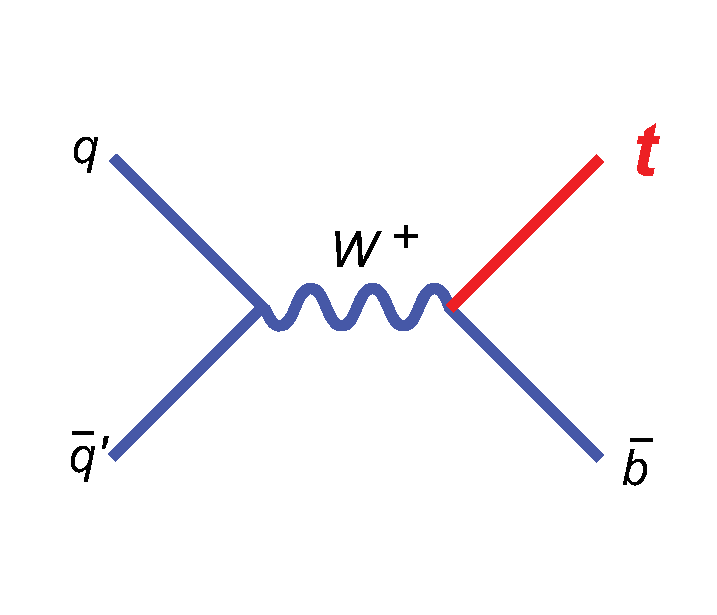
\includegraphics[width=0.25\textwidth]{eps/Theory/feynman_tb_note.eps}
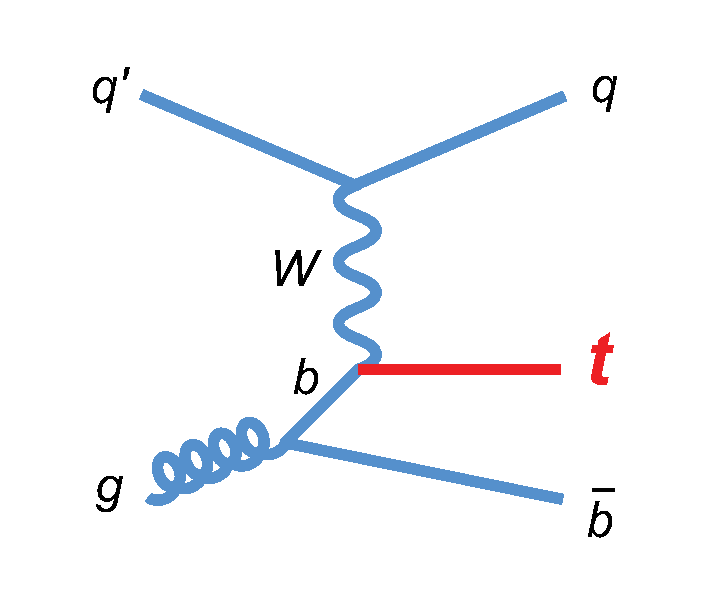
\includegraphics[width=0.25\textwidth]{eps/Theory/feynman_tqb_note.eps}
\end{center}
\caption{Feynman diagrams for the $s$-channel ``tb'' (left) and $t$-channel ``tqb'' (right) single top production mode.}
\label{singletop}
\end{figure}

Measuring single top quark production is interesting because one can directly determine the magnitude of the CKM matrix element $V_{tb}$ since $\sigma_{tb+tqb}\propto|V_{tb}|^{2}$. Single top quark production is also sensitive to new physics. The existence of a new charged gauge boson ($W^{'}$) would enhance the effective $s$-channel cross section, while flavor changing neutral currents in the top sector would enhance the measured $t$-channel cross section.

We select single-top-like data events with a final state signature of one high $p_{T}$ lepton, large missing $E_{T}$, and two to four jets. In this decay channel the major backgrounds are $W$+jets and $\ttbar$ production with a signal-to-background ratio of 1:20~after event selection. To enhance the single top quark signal a technique known as the matrix element method is employed, which uses leading order matrix elements to compute an event probability for both signal and background hypotheses. A discriminant is created from these probabilities, which shows excellent separation of single top signal from the backgrounds. The single top cross section is extracted using a Bayesian binned likelihood approach based on the matrix element discriminant. Using the expected signal acceptance, background, and observed data we measure the single top quark cross section:
$$
\begin{array}{lll}
\sigma\left({\ppbar}{\rargap}tb+tqb+X\right) = 4.6 ^{+1.8}_{-1.5}~{\rm pb}\\
\end{array}
$$
The probability for the background to have fluctuated up to give at
least the cross section measured in this analysis is
$0.21\%$, which corresponds to a Gaussian equivalent significance of
$2.9\sigma$.

This analysis is one of three single top searches performed by the $\dzero$~collaboration. These analyses are combined using the BLUE (Best Linear Unbiased Estimator) method; this results in a measured cross section of $4.8\pm1.3$~pb with $3.5\sigma$ signal significance providing evidence for single top quark production. 

I will also present the result of a search for W-associated Higgs production. This production channel, whose Feynman diagram is shown in Figure~\ref{wh}, is one of most sensitive channels for a low mass ($m_{H}<135$~GeV) Standard Model Higgs. 

\begin{figure}[!h!tbp]
\begin{center}
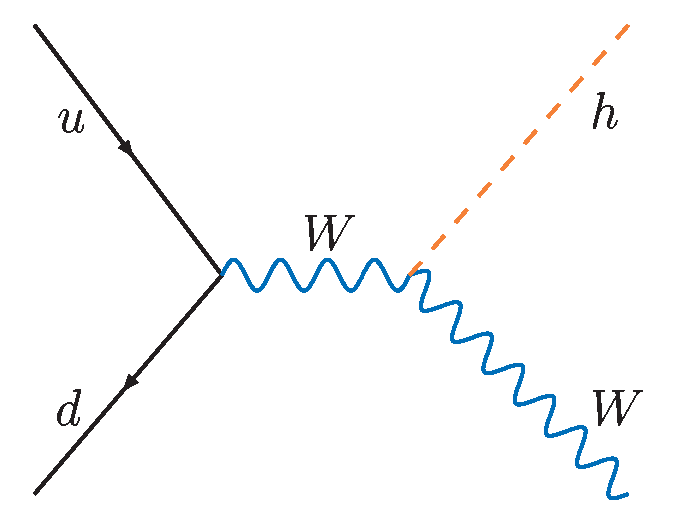
\includegraphics[width=0.25\textwidth]{eps/Feynman/wh.eps}
\end{center}
\caption{Feynman diagrams for the W-associated Higgs production channel.}
\label{wh}
\end{figure}

Using the same dataset and the matrix element analysis technique, we did not observe and excess of data above background and therefore set limits on the WH cross section. Since the Higgs mass is unknown the cross section limits are given for six mass points ranging from 105 to 155~GeV. For a Higgs mass of 115~GeV we measure a 95\% CL upper limits for $\sigma_{WH}\times\rm{BR}(H\rightarrow b\bar{b}) < 1.74$~pb, which is a factor of 13 larger than the expected Standard Model cross section.

 \end{document}